\documentclass[conference]{IEEEtran}
\IEEEoverridecommandlockouts
% The preceding line is only needed to identify funding in the first footnote. If that is unneeded, please comment it out.
\usepackage{cite}
\usepackage{amsmath,amssymb,amsfonts}
\usepackage{algorithmic}
\usepackage{graphicx}
\usepackage{textcomp}
\usepackage{xcolor}
\def\BibTeX{{\rm B\kern-.05em{\sc i\kern-.025em b}\kern-.08em
    T\kern-.1667em\lower.7ex\hbox{E}\kern-.125emX}}
\begin{document}

\title{SafeDetect Product Documentation\\
%{\footnotesize \textsuperscript{*}Note: Sub-titles are not captured in Xplore and
%should not be used}
}

\author{\IEEEauthorblockN{1\textsuperscript{st} Charles Andre}
\IEEEauthorblockA{\textit{Ming Hsieh Department of Electrical Engineering} \\
\textit{University of Southern California}\\
Los Angeles, USA \\
candre@usc.edu}
\and
\IEEEauthorblockN{2\textsuperscript{nd} Yutong Gu}
\IEEEauthorblockA{\textit{Ming Hsieh Department of Electrical Engineering} \\
\textit{University of Southern California}\\
Los Angeles, USA \\
yutonggu@usc.edu}
\and
\IEEEauthorblockN{3\textsuperscript{rd} Sharon Guo}
\IEEEauthorblockA{\textit{Ming Hsieh Department of Electrical Engineering} \\
\textit{University of Southern California}\\
Los Angeles, USA  \\
guox@usc.edu}
\and
\IEEEauthorblockN{4\textsuperscript{th} Sufyan Shaikh}
\IEEEauthorblockA{\textit{Ming Hsieh Department of Electrical Engineering} \\
\textit{University of Southern California}\\
Los Angeles, USA  \\
sufyansh@usc.edu}

}

\maketitle

\begin{abstract}
SafeDetect is a product developed over the course of the University of Southern California's Internet and Cloud Computing course. By utilizing an audio detector, multitech xdot, raspberry pi, AWS and a machine learning model we are able to detect gunshots and triangulate their location. This paper will go over motivation, implementation, and results.
\end{abstract}

%\begin{IEEEkeywords}
%component, formatting, style, styling, insert
%\end{IEEEkeywords}

\section{Introduction}
Gun violence, specifically death from gun violence, has been steadily increasing over the past few decades. When a person is shot they must receive urgent medical treatment in order to mazimize their chances of survival. In the past pedestrians are often relied on to report cases of gun violence and only then are police and medical professionals alerted to report to the scene. This delay and reliance on human intervention can lead to delay in medical help. In the worst case a treatable wound may turn fatal.

In this paper we propose SafeDetect as an alternative that will rely on audio detection rather than human intervention. By removing the human component our system will have faster response time and will be able to avoid situations where a person is shot and no one is aware. Our product works as a network system where multiple units collaborate to both detect gunshots and use their locations to triangulate the location of the shooting.

\subsection{Current Market}

Smart gunshot detection systems are becoming increasingly common in urban cities. Large cities like Los Angeles have a policing budget of over four million and currently employees a gun detection system with a high false positive rate and a 40 second delay. Cities are willing to pay and have been paying for smart gunshot systems.

Durham, North Carolina received a proposal from a competitor to install gunshot detection technology in a three mile radius. Twenty to twenty-five sensors would be instaled per square mile. Initial annual cost was estimate to be \$235,000 and then \$195,000 annually thereafter.
If we had submitted our product in the same proposal we would be able to place two-hundred nodes and remain significantly cheaper with an approximate initial annual setup of \$50,000 and approximately \$2,000 annually thereafter. This is with no return profit butwe have enough leeway to scale up our pricing for profit and still remain below our competitor

\section{Target Problem}

In order to implement successful and useful gunshot detection our system will focus on acheving two main goals.
\begin{enumerate}
\item Detecting when a gunshot has occured.
\item Tracing the location of the gunshot.
\end{enumerate}


\section{System Overiview}

Here we will discuss the technical implementation of our product. It is a network of several individual nodes centered around a receiving Mulitech Conduit. 



\subsection{Individual Module Overview}

Each node will have a unique identifier and three main physical components.
\begin{figure}[htbp]
\centerline{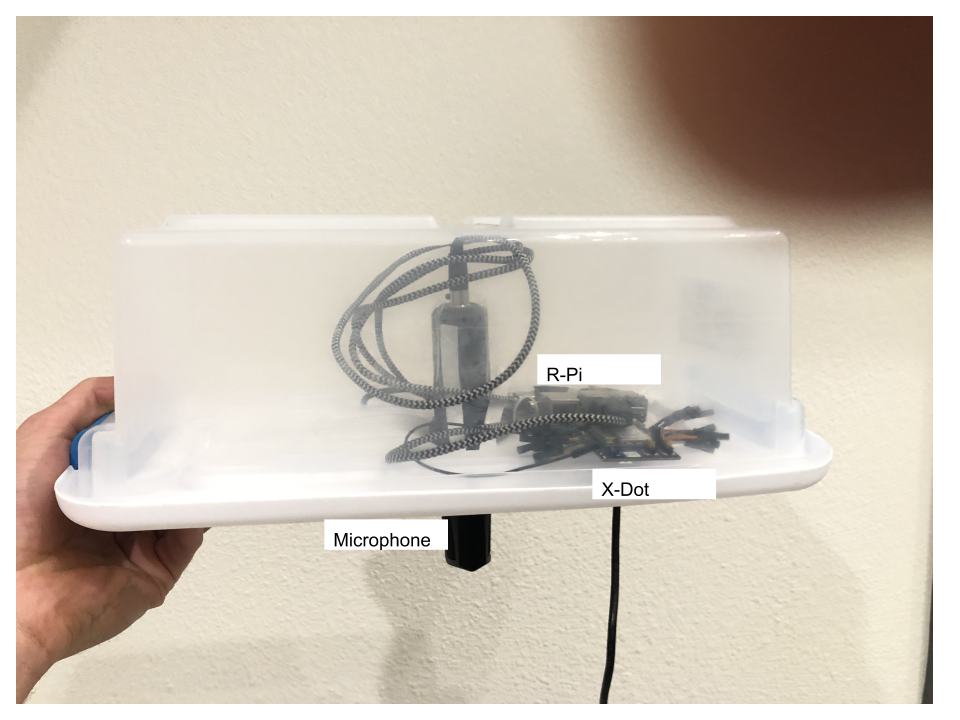
\includegraphics[width=0.7\columnwidth]{physical_system_box.png}}
\caption{Physical components assembled attached to lid of a box.}
\label{fig}
\end{figure}
\begin{figure}[htbp]
\centerline{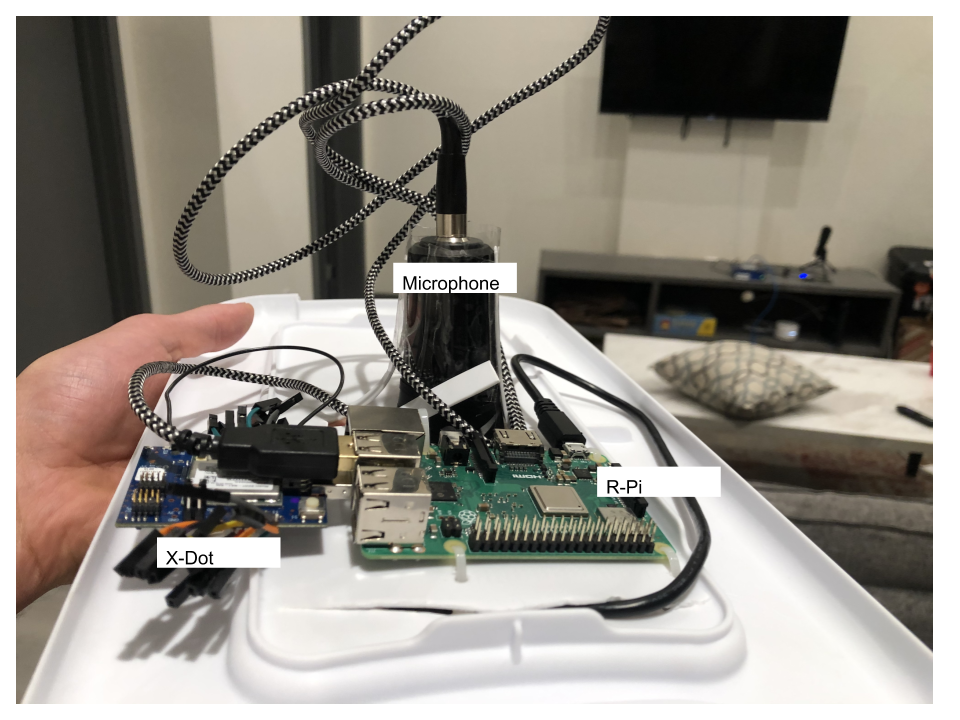
\includegraphics[width=0.7\columnwidth]{physical_system.png}}
\caption{Physical components assembled attached to lid of a box.}
\label{fig}
\end{figure}
\begin{enumerate}
\item Microphone Audio Sensor 
\item Raspberry pi
\item Multitech xDot

\end{enumerate}

The microphone is constantly recording audio and storing it in the Raspberry pi. Once the audio reaches the raspberry pi, the pi will constantly be scanning for if audio amplitute exceeds a certain threshold. This threshold is determined from extensive trial and error. It is high enough that normal, everyday activity does not trigger it but not so high that it can not detect gunshots from afar. 
Once the threshold is surpassed the current audio stored in the raspberry pi will be processed and sent through our machine learning model to see if a gunshot is detected. The pi will containing storing audio in the background so that there are no audio gaps.

If a gunshot was indeed heard than that information is sent to the xDot over a USB serial port. The xDot will then send the information over to the multitech conduit over lora.

\subsection{Network Overview}
A single network consists of serveral individual nodes around a multitech conduit pre-loaded with Node-red. The conduit receives two main pieces of information from the xDots over lora radio: whether or not a gunshot was detected and the pi's local timestamp. By sending data over lora radio instead of another method like wifi we get two main benefits.
 
\begin{itemize}
\item Higher Range\\  Lora signals have a range of 10 km if there is direct line of sight. 
We would be able to acheive that line of sight because our product will be placed high up out of the way of everyday life. In more suburban areas where less units may be required we are able to space out our nodes more while staying in range of the conduit.
\item Lower Costs \\ Other competing systems often utilizes wifi to send their data. This leads to a higher recurring cost.

\end{itemize}

On node-red the data is converted to a json object and then sent to the cloud. The only requirement to connect to the cloud is to create a HTTP request node with the URL being the endpoint from the AWS account
\section{AWS Cloud Overview}

Our project makes use of a handful of AWS applications, primarily IoT Core, Lambda, and S3. IoT Core is an application that receives messages from IoTs and publishes those messages to an MQTT topic. Lambda is an event-driven, serverless computing platform provided by Amazon as a part of Amazon Web Services. It is a computing service that runs code in response to events and automatically manages the computing resources required by that code. S3, or Simple Storage Service, is a service offered by AWS that provides object storage through a web interface. 

Data from the conduit is passed over to IoT Core. In the IoT Core all messages sent by the xDot are available in the topic in JSON format. The object contains the device’s embedded unique ID (EUI), timestamp, gun-shot confidence and the volume. However, these messages are not saved by default and need to be saved into S3. To save messages into S3, we invoke a rule, that saves a given message to S3. It is possible to save the files such that the files are named [Device EUI].json. By doing this, all messages stored in the S3 Bucket are current JSON objects and this allows us to iteratively search through the bucket. Searching through all the JSON files allows us to find the three nodes that heard the gunshots first to pinpoint the location of the gunshot.

\subsection {Multilateration}
To pinpoint the location of the gunshot, we need to run a function. Lambda is perfect for this because it can be set to only activate based on a trigger. The trigger is a condition that, if met, calls the function, giving us our desired output. The trigger we set is that if a gunshot message is heard on IoT Core, activate the lambda function. Our function iteratively finds the three nodes that heard it the soonest and grabs the timestamp and EUI of the nodes. The location of the nodes is saved in a lookup table referenced by the EUI. By using the EUIs, we can find the GPS location of the nodes that heard the gunshot. The GPS location is in standard WGS84 format and is then converted to Cartesian coordinates. After converting the coordinates, we run a multilateration algorithm based on Bancroft’s Algorithm [] . This algorithm makes use of differences in Times of Arrival (TOA) of a signal and locations of base stations (our nodes) to pinpoint the location of the sender of the signal. In our case, the signal is a sound wave and the velocity of a sound wave is 343 m/s. By using this, we can accurately obtain the Cartesian coordinates of where the sound originated and convert it back to GPS coordinates.


\section{Time Synchronization}
Initially, we were going to use the built in time stamps that go along with the LoRaWAN protocol. However, we soon realized that there could be inaccuracies on the order of seconds due to where the gunshot lies in the sliding window. If by chance, the gunshot is at the start of the window on one node and the end of a window on another node, we would detect a multiple second time difference, which is incorrect. 

To fix this, we normalize the clock on the Raspberry Pi to the Master clock running on AWS. To do this, we send the Raspberry pi time almost instantaneously, and at least with equal delay at every node, to the conduit. There we calculate the time difference between that node’s time and the master time. We store this conversion factor in a lookup table, which allows for easy conversion to real time whenever we receive a Raspberry Pi time stamped message. The Raspberry Pi stamps a window with the time at which the peak sound (assumed to be the gunshot) was detected.

\section{Results}

\subsection{Figures and Tables}
\paragraph{Positioning Figures and Tables} Place figures and tables at the top and 
bottom of columns. Avoid placing them in the middle of columns. Large 
figures and tables may span across both columns. Figure captions should be 
below the figures; table heads should appear above the tables. Insert 
figures and tables after they are cited in the text. Use the abbreviation 
``Fig.~\ref{fig}'', even at the beginning of a sentence.

\begin{table}[htbp]
\caption{Table Type Styles}
\begin{center}
\begin{tabular}{|c|c|c|c|}
\hline
\textbf{Table}&\multicolumn{3}{|c|}{\textbf{Table Column Head}} \\
\cline{2-4} 
\textbf{Head} & \textbf{\textit{Table column subhead}}& \textbf{\textit{Subhead}}& \textbf{\textit{Subhead}} \\
\hline
copy& More table copy$^{\mathrm{a}}$& &  \\
\hline
\multicolumn{4}{l}{$^{\mathrm{a}}$Sample of a Table footnote.}
\end{tabular}
\label{tab1}
\end{center}
\end{table}



Figure Labels: Use 8 point Times New Roman for Figure labels. Use words 
rather than symbols or abbreviations when writing Figure axis labels to 
avoid confusing the reader. As an example, write the quantity 
``Magnetization'', or ``Magnetization, M'', not just ``M''. If including 
units in the label, present them within parentheses. Do not label axes only 
with units. In the example, write ``Magnetization (A/m)'' or ``Magnetization 
\{A[m(1)]\}'', not just ``A/m''. Do not label axes with a ratio of 
quantities and units. For example, write ``Temperature (K)'', not 
``Temperature/K''.

\section*{Acknowledgment}

We would like to acknowledge our Internet and Cloud Computiong Professor, Dr. Young Cho and our Internet and Cloud Computing  Teaching Assistant Arthur Win.

\section*{References}

Please number citations consecutively within brackets \cite{b1}. The 
sentence punctuation follows the bracket \cite{b2}. Refer simply to the reference 
number, as in \cite{b3}---do not use ``Ref. \cite{b3}'' or ``reference \cite{b3}'' except at 
the beginning of a sentence: ``Reference \cite{b3} was the first $\ldots$''

Number footnotes separately in superscripts. Place the actual footnote at 
the bottom of the column in which it was cited. Do not put footnotes in the 
abstract or reference list. Use letters for table footnotes.

Unless there are six authors or more give all authors' names; do not use 
``et al.''. Papers that have not been published, even if they have been 
submitted for publication, should be cited as ``unpublished'' \cite{b4}. Papers 
that have been accepted for publication should be cited as ``in press'' \cite{b5}. 
Capitalize only the first word in a paper title, except for proper nouns and 
element symbols.

For papers published in translation journals, please give the English 
citation first, followed by the original foreign-language citation \cite{b6}.

\begin{thebibliography}{00}
\bibitem{b1} G. Eason, B. Noble, and I. N. Sneddon, ``On certain integrals of Lipschitz-Hankel type involving products of Bessel functions,'' Phil. Trans. Roy. Soc. London, vol. A247, pp. 529--551, April 1955.
\bibitem{b2} J. Clerk Maxwell, A Treatise on Electricity and Magnetism, 3rd ed., vol. 2. Oxford: Clarendon, 1892, pp.68--73.
\bibitem{b3} I. S. Jacobs and C. P. Bean, ``Fine particles, thin films and exchange anisotropy,'' in Magnetism, vol. III, G. T. Rado and H. Suhl, Eds. New York: Academic, 1963, pp. 271--350.
\bibitem{b4} K. Elissa, ``Title of paper if known,'' unpublished.
\bibitem{b5} R. Nicole, ``Title of paper with only first word capitalized,'' J. Name Stand. Abbrev., in press.
\bibitem{b6} Y. Yorozu, M. Hirano, K. Oka, and Y. Tagawa, ``Electron spectroscopy studies on magneto-optical media and plastic substrate interface,'' IEEE Transl. J. Magn. Japan, vol. 2, pp. 740--741, August 1987 [Digests 9th Annual Conf. Magnetics Japan, p. 301, 1982].
\bibitem{b7} M. Young, The Technical Writer's Handbook. Mill Valley, CA: University Science, 1989.
\end{thebibliography}

\end{document}